\documentclass[a4paper, 12pt]{article}
\usepackage{amssymb}
\usepackage{amsmath}
\usepackage{verbatim}
\setcounter{tocdepth}{3}
\usepackage{graphicx}
\usepackage{afterpage}
\usepackage{floatpag}
\usepackage{setspace}
\floatpagestyle{empty}
%\usepackage[a4paper, total={4in, 6in},margin=4in]{geometry}
\usepackage[export]{adjustbox}
%\usepackage[paperwidth=7.0in, paperheight=10.7in]{geometry}
%\usepackage{layout}
%\layout{layoutwidth=180mm,layoutheight=227mm}
%\geometry{a4paper,left=25mm,right=25mm,top=25mm,bottom=25mm,heightrounded}
%\usepackage[a4paper]{geometry}
\usepackage{listings}
\usepackage{subfigure}
\usepackage{wrapfig}
\usepackage[hyperindex=false,colorlinks=false]{hyperref}
\usepackage{fullpage}
\usepackage{tikz}
\usetikzlibrary{shapes.geometric, arrows}
\DeclareMathSizes{20}{20}{20}{20}

\tikzstyle{startstop}=[rectangle, rounded corners, minimum width=3cm, minimum height=1cm, text centered, text width=4cm, draw=black,fill=red!30]

\tikzstyle{io}=[trapezium, trapezium left angle=70, trapezium right angle=110, minimum width=3cm, minimum height=1cm, text centered, text width=4cm, draw=black, fill=blue!30]

\tikzstyle{process}=[rectangle, minimum width=3cm, minimum height=1cm, text centered, text width=4cm, draw=black,fill=orange!30]

\tikzstyle{decision}=[diamond, minimum width=3cm, minimum height=1cm, text centered, text width=4cm, draw=black, fill=green!30]

\tikzstyle{arrow}=[thick,->,>=stealth]

\begin{document}

\begin{titlepage}

%\newcommand{\HRule}{\rule{\linewidth}{0.5mm}} % Defines a new command for the horizontal lines, change thickness here
\newcommand{\HRule}{\rule{155mm}{0.5mm}} % Defines a new command for the horizontal lines, change thickness here

\center % Center everything on the page

%----------------------------------------------------------------------------------------
%   HEADING SECTIONS
%----------------------------------------------------------------------------------------

\textsc{\LARGE Technische Universit{\"a}t M{\"u}nchen}\\[1.5cm] % Name of your university/college
\textsc{\Large Chair For Computer Technology and Computer Organisation}\\[0.5cm] % Major heading such as course name

%----------------------------------------------------------------------------------------
%   TITLE SECTION
%----------------------------------------------------------------------------------------
\vspace{30mm}
\begin{center}
\Large\textit{Guided Research}
\end{center}
\HRule \\[0.4cm]
{ \Large \bfseries A Protocol for the Integration of Invasive Resource Management into Standard Batch Schedulers}\\[0.5cm] % Title of your document
\HRule \\[1.5cm]

%----------------------------------------------------------------------------------------
%   AUTHOR SECTION
%----------------------------------------------------------------------------------------
\vspace{48mm}
\begin{minipage}{0.4\textwidth}
\begin{flushleft} \large
\emph{Student:}\\
Nishanth Nagendra % Your name
\end{flushleft}
\end{minipage}
\begin{minipage}{0.4\textwidth} 
\begin{flushright} \large
\emph{Supervisor:} \\
Prof. Dr. Michael Gerndt \\~\\ % Supervisor's Name
\emph{Advisor:} \\
M.Sc. Isaias Alberto Compres Urena  % Advisor's Name
\end{flushright}
\end{minipage}\\[2cm]

% If you don't want a supervisor, uncomment the two lines below and remove the section above
%\Large \emph{Author:}\\
%John \textsc{Smith}\\[3cm] % Your name

%----------------------------------------------------------------------------------------
%   DATE SECTION
%----------------------------------------------------------------------------------------

{\large \today}\\[2cm] % Date, change the \today to a set date if you want to be precise

\end{titlepage}

\begin{center}
\huge \bfseries Acknowledgement
\end{center}
\thispagestyle{empty}
\vspace{35mm}
I would like to thank  Isaias for his constant support and guidance throughout the guided research especially when I faced some challenges in understanding certain topics. I would also like to thank Prof. Dr. Michael Gerndt for providing me with this opportunity to work on such an interesting topic.

\newpage

\begin{center}
\huge \bfseries Abstract
\end{center}
\thispagestyle{empty}
\vspace{35mm}

Invasive computing is a novel paradigm for the design and resource-aware programming of future parallel computing systems. It enables the programmer to write resource aware programs and the goal is to optimize the program for the available resources. Traditionally, parallel applications implemented using MPI are executed with a fixed number of MPI processes before submitting to a HPC(High Performance Computing) system. This results in a fixed allocation of resources for the job. Newer techniques in scientific computing such as AMR(Adaptive mesh refinement) result in applications exhibiting complex behavior where their resource requirements change during execution. Invasive MPI which is a part of an ongoing research effort to provide MPI extensions for the development of Invasive MPI applications will result in evolving jobs for the HPC systems at runtime supporting such AMR techniques. Unfortunately, using only static allocations result in the evolving applications being forced to execute using their maximum resource requirements that may lead to an inefficient resource utilisation. In order to support such parallel evolving applications at HPC centers there is an urgent need to investigate and implement extensions to existing resource management systems or develop an entirely new one. These supporting infrastructures must be able to handle these evolving jobs and also the legacy rigid jobs intelligently and hence newer protocols for integration of such invasive resource management into existing standard batch systems needs to be now explored.

\newpage
\thispagestyle{empty}
\tableofcontents
\newpage

\setcounter{page}{1}
\section{Introduction}
Invasive computing is a novel paradigm for the design and resource-aware programming of future parallel computing systems. It enables the programmer to write efficient resource aware programs. This approach can be used to allocate, execute on and free resources during execution of the program. HPC infrastructure like Clusters, Supercomputers execute a vast variety of jobs, majority of which are parallel applications. These centers use intelligent resource management systems that should not only perform tasks of job management, resource management and scheduling but also satisfy important metrics like higher system utilization, job throughput and responsiveness. Traditionally, MPI applications are executed with a fixed number of MPI processes but with Invasive MPI they can evolve dynamically at runtime in the number of their MPI processes. This in turn supports advanced techniques like AMR where the working set size of applications change at runtime. These advancements entail an immediate need for stronger and intelligent resource management systems that can provide efficient resource utilization at HPC centers. They should also now be able to achieve much higher system utilisation, energy efficiency etc. compared to their predecessors due to elasticity of the applications.\par
\noindent
\\Under the collaborative research project funded by the German research foundation(DFG) in the Transregional Collaborative Research Centre 89(TRR89), research efforts are being made to investigate Invasive computing approach vertically at different levels of abstraction right from the hardware up to the programming model. Invasive MPI is one such effort towards invasive programming with MPI where the application programmer has MPI extensions available using which he/she can specify at certain safe points in the program to allow for elasticity which means the application can evolve.

\subsection{Resource Management}
In order to support such parallel evolving applications at HPC centers there is an urgent need to investigate and implement extensions to existing resource management systems or develop an entirely new one. These supporting infrastructures must be able to handle the new kind of evolving jobs/applications and the legacy rigid jobs intelligently keeping in mind that they should now be able to achieve much higher system utilisation, energy efficiency etc compared to their predecessors due to the elasticity of the applications. Two of the most widely used resource managers on HPC systems are SLURM and TORQUE. The 2 major components in general of any sophisticated resource manager are the batch scheduler and the process manager.
\subsection{Batch Scheduling}
The batch scheduler accepts job descriptions given by end users some of which mention as to how long the job would run and the amount of resources it will need. It maintains a queue of jobs and dispatches them to the process manager based on some criteria and algorithms. The decisions made depend on the state of resources and also others like job priorities, fairness, waiting times etc. The process manager on the other hand has lesser intelligence and does the task of mapping the processes of a parallel application on the hardware based on the node list provided to it by the batch scheduler. In the context of invasive computing we need to be investigate for new requirements in the interaction between the batch scheduler and process manager. The decisions made by the batch scheduler need to be influenced to support evolving jobs.\par
\noindent
\\In contrast to the earlier uni-directional communication from batch scheduler to process manager, we now need to support a bi-directional communication between the two. The capabilities of existing batch schedulers could be leveraged rather than having to replace an entire system with a new one. The possiblity of supporting a new interface for the existing batch scheduler needs to be explored such that it communicates with a new invasive process management that controls a dedicated partition to support invasive computing. An investigation needs to be done on whether the existing interface of batch schedulers towards process manager could be extended or re-used and also on the possiblity of receiving feedback from the invasive process manager to allow the batch scheduler to be influenced. The invasive process manager one level below in the hierarchy as shown in the figure below will work on local metrics of the dedicated invasive partition within the cluster allocated by the batch scheduler.\par
\noindent
\\The investigations of this guided research are an initial study that will support the continuing research effort for developing Invasive MPI and extended resource management systems to support Invasive computing systems.

\subsection{Software Requirements}
\newpage
\section{Invasive Computing}
The throughput of supercomputers depends not only on efficient job scheduling but also on the type of jobs that form the workload. Malleable jobs are most favourable for a cluster as they can dynamically adapt to a changing allocation of resources. The batch system can expand or shrink a running malleable job to improve system utilization, throughput, and response times. In the past, however the rigid nature of commonly used programming models like MPI made writing malleable applications a daunting task, which is why it remains largely unrealized. This is now changing. To improve fault tolerance, load imbalance, and energy efficiency in emerging exascale systems more adaptive programming paradigms are being investigated. Although they may offer better support for malleability, current batch systems still lack management facilities for malleable jobs and are therefore incapable of leveraging their potential. In this guided research we propose an extension to the SLURM resource manager to support malleable jobs.
\subsection{Job Classification}
As defined by Feitelson and Rudolph [1], jobs can be classified into four categories based on their flexibility.
\begin{itemize}
\item \textbf{\textit{Rigid job:}} This is the most common type which requires a fixed number of processors throughout its execution.
\item \textbf{\textit{Moldable job:}} In this kind of job the resource set can be molded or modified by the batch system before starting the job (e.g. to effectively fit alongside other rigid jobs). Once started its resource set cannot be changed anymore.
\item \textbf{\textit{Evolving job:}} These kind of jobs request for resource expansion or shrinkage during their execution. Applications that use multiscale analysis like Quadflow or Adaptive mesh refinement(AMR) exhibit this kind of behavior typically due to unexpected increases in computations or having reached hardware limits(e.g. memory) on a node. 
\item \textbf{\textit{Malleable job:}} The expansion and shrinkage of resources are initiated by the batch system in contrast to the evolving jobs. The application adapts itself to the changing resource set.
\end{itemize}
The first two types fall into the category of what is called as the static allocation since the allocation of rigid and moldable jobs must be finalized before the job starts. Whereas, the last two types fall under the category of dynamic allocation since this property of expanding or shrinking evolving and malleable jobs(together termed adaptive jobs) happens at runtime.\par
\noindent
\\
Malleable jobs hold a strong potential to obtain high system performance. Batch systems can substantially improve the system utilization, throughput and response times with efficient shrink/expand strategies for malleable jobs. Similarly, applications also profit when expanded with additional resources as this can increase application speedup and improve load balance across the job’s resource set. Enabling malleable jobs in cluster systems requires three major components: (i) a parallel runtime that is able to adapt to a changing resource set, (ii) a batch system with dynamic allocation facilities, and (iii) a communication mechanism between the two. Traditionally, all batch systems support only static allocations.\par

\subsection{Traditional Resource Management}
The role of a resource manager is that it acts like a \textit{glue} for a parallel computer to execute parallel jobs. It should make a parallel computer as easy to use as almost a PC. MPI would typically be used to manage communications within the parallel program. A resource manager allocates resources within a cluster, launches and otherwise manages jobs. Some of the examples of widely used open source as well as commercial resource managers are \textbf{SLURM, TORQUE, OMEGA, IBM Platform LSF} etc. Together with a scheduler it is termed as a \textbf{\textit{Batch System}}. The Batch System serves as a middleware for managing supercomputing resources. The combination of \textit{Scheduler}$+$\textit{Resource Manager} makes it possible to run parallel jobs.\par
\noindent
\\
The role of a job scheduler is to manage queue(s) of work when there is more work than resources. It supports complex scheduling algorithms which are optimized for network topology, energy efficiency, fair share scheduling, advanced reservations, preemption, gang scheduling(time-slicing jobs) etc. It also supports resource limits(by queue, user, group, etc.). Many batch systems provide both resource management and job scheduling within a single product (e.g. LSF) while others use distinct products(e.g. Torque resource manager and Moab job scheduler). Some other examples of Job scheduling systems are \textbf{LoadLeveler, OAR, Maui, SLURM} etc.\par
\noindent
\\
The prime focus of this work will be on SLURM(Simple Linux Utility For Resource Management) which will be the choice of batch system upon which the support for Invasive Computing will be demonstrated. SLURM is a sophisticated open source batch system with about 500,000 lines of C code whose development started in the year 2002 at Lawrence Livermore National Laboratory as a simple resource manager for Linux Clusters and a few years ago spawned into an independent firm under the name SchedMD. SLURM has since its inception also evolved into a very capable job scheduler through the use of optional plugins. It is used on many of the world's largest supercomputers and is used by a large fraction of the world's TOP500 Supercomputer list. It supports many UNIX falvors like AIX, Linux, Solaris and is also fault tolerant, highly scalable, and portable.\par
\noindent
\\
Plugins are dynamically linked objects loaded at run time based upon configuration file and/or user options. Approximately $80$ plugins of different varities are currently available. Some of them are listed below:\\
\begin{itemize}
\item Accounting storage: MySQL, PostgreSQL, textfile.
\item Network Topology: 3D-Torus, tree.
\item MPI: OpenMPI, MPICH1, MVAPICH, MPICH2, etc.
\end{itemize} 
PLugins are typically loaded when the daemon or command starts and persist indefinitely. They provide a level of indirection to a configurable underlying function.
\begin{figure}[h]
\centering
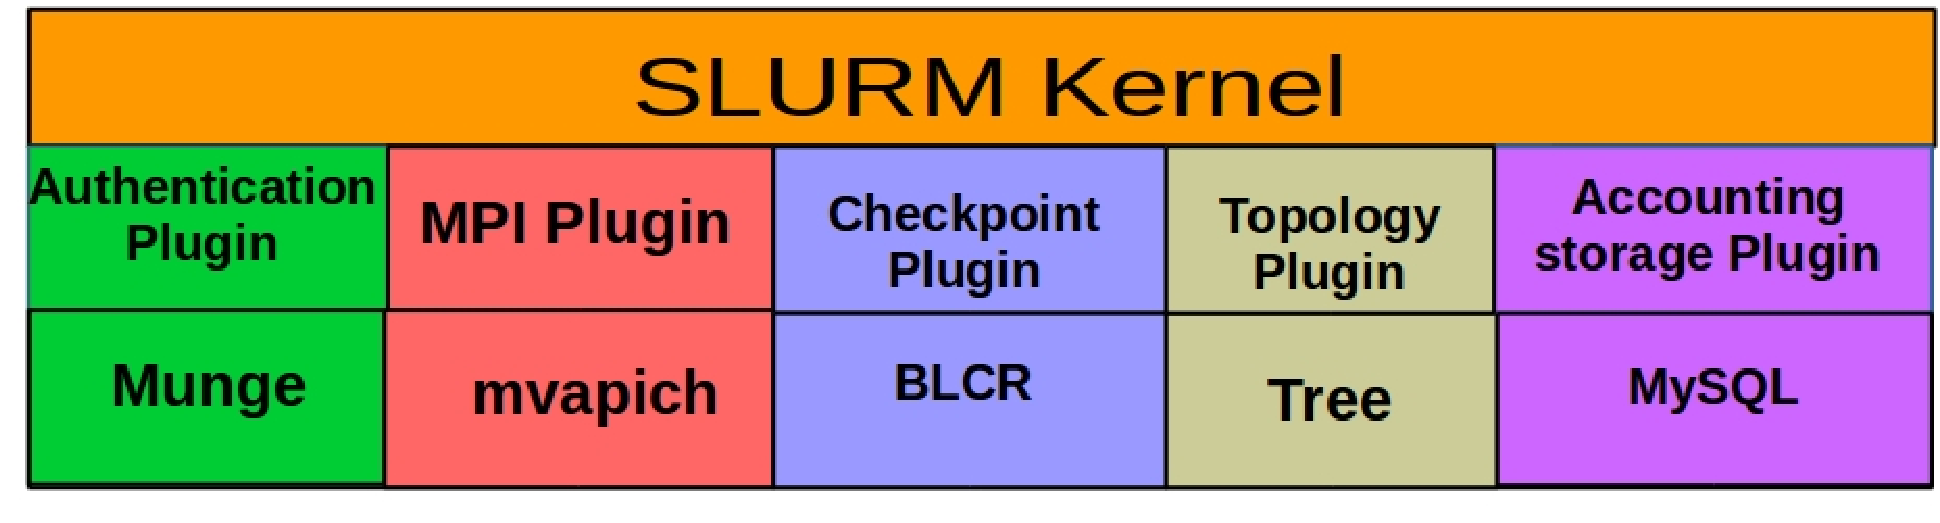
\includegraphics[width=1.0\textwidth]{./plugin.eps}
\vspace{-0.15in}
\caption{Software layers of SLURM}
\label{fig:6}
\end{figure}
\subsection{Support For Invasive Computing}
Modern heuristic techniques, also called metaheuristics are a family of procedures which benefit from some sort of intelligence in their search for finding the solution to a problem. It is a higher level procedure designed to find, generate, or select a heuristic(partial search algorithm) that may provide a sufficiently good solution to an optimization problem, especially with incomplete or imperfect information or limited computation capacity. They may not provide optimal solution but they provide a sufficiently good solution rapidly and effectively. Simulated annealing, genetic algorithm, tabu search, neural network, ant system are some examples of such meta heuristics.\par
\noindent
\\This project implements the genetic algorithm on DNDP. Genetic algorithm (GA) is a search heuristic that mimics the process of natural selection. This heuristic (also sometimes called a metaheuristic) is routinely used to generate useful solutions to optimization and search problems.[1] Genetic algorithms belong to the larger class of evolutionary algorithms (EA), which generate solutions to optimization problems using techniques inspired by natural evolution, such as inheritance, mutation, selection, and crossover. Genetic algorithms find application in bioinformatics, phylogenetics, computational science, signal and image processing, Bayesian inference, machine learning, risk analysis and rare event sampling, Engineering and robotics, economics, manufacturing, mathematics, mathematical finance, molecular chemistry, computational physics, pharmacokinetic, pharmacometrics, and other fields.\par
%\noindent
\clearpage
\section{Design and Implementation}
This section describes a high level design of the software implemented with the help of flow charts and pseudo code. Follwed by this is a small snapshot of certain low level details of the software that will help the reader to understand as to what functionalities this software offers in a summary.
\subsection{Software Architecture}
The following page shows the software architecture of how Invasive Resource Management can be supported with a traditional resource manager and how exactly the new software components will fit in the existing software hierarchy. The figure [X] relates closely to how SLURM is organized since the intention of this work would be to demonstrate the support for Invasive Computing with the help of SLURM as a resource manager.
\begin{itemize}
\item The top layer is that of the core resource management component which has access to job queues. In this architecture, it will now have access to not only the queue for the legacy(static) jobs but also invasive job queue(jobs submittted to invasic partition that supports invasive computing).
\item In a traditional setup the top layer will perform the task of job scheduling as well. This means that it will select a job(s) from the queue of jobs based on the current state of resources and many other factors to dispatch it to the traditional process manager below in the hierarchy. The process manager then takes the responsibility of launching these jobs on the allocated resources in the partition and managing them for their full lifetime. In case of parallel jobs, it will again manage the job in a parallel environment along with facilitating the communication amongst the parallel tasks/processes with the help of a PMI(Process Manager Interface) server. In the process of managing these jobs, the process manager may also spawn slave daemons on each of the nodes which are a part of the resource allocation for a single job to manage them more effectively.
\item Depending on the resource manager which will be used to support this invasive computing, a new scheduler specifically for invasive jobs needs to be integrated into it. In case of SLURM which has a modular design with several optional plugins, a new plugin by name "iScheduler" will be implemented inside the core component of SLURM to handle job scheduling.
\item As discussed in the previous chapter, an independent Invasive resource management component by the name "iHypervisor" will be implemented which needs to communicate with this new scheduling component iScheduler and influence the scheduling decisions taken by it. The iHypervisor sits between the top layer and the invasive partition.
\item .
\end{itemize}
\clearpage
\begin{figure}[h]
\centering
\vspace{-0.15in}
\includegraphics[width=1.0\textwidth, height=225mm]{"software architecture".eps}
\caption{Invasive Resource Management Architecture}
\label{fig:7}
\end{figure}
%\begin{minipage}[t]
%\vspace{0mm}
%\afterpage{
%\begin{figure}[htbp]
%\floatpagestyle{empty}
%\hspace*{-0.3in}
%\raisebox{12mm}{
%\includegraphics[scale=0.95]{./diagram.eps}%}
%\caption{\textbf{Flow chart of the software imlementation}}
%\label{fig 1}
%\end{figure}
%}
%\end{minipage}[t]
%\afterpage%{
%\thispagestyle{empty}
%\begin{figure}[htbp]
%\floatpagestyle{empty}
%\hspace*{0.1in}
%\includegraphics[scale=0.9]{./diagram1.eps}
%\caption{\textbf{Pseudo code for algorithms}}
%\label{fig 2}
%\end{figure}
%}
%\afterpage{
%\thispagestyle{empty}
%\begin{figure}[htbp]
%\floatpagestyle{empty}
%\hspace*{-0.10in}
%\includegraphics[scale=0.85]{./diagram2.eps}
%\caption{\textbf{Pseudo code for algorithms}}
%\label{fig 3}
%\end{figure}
%}
\clearpage
\subsection{Protocols}
\begin{itemize}
\item \textbf{\textit{Protocol Initialization:}}
\item \textbf{\textit{Protocol Finalization:}}
\item \textbf{\textit{Negotiation:}}
\item \textbf{\textit{Feedback:}}
\item \textbf{\textit{Urgent Jobs:}}
\end{itemize}
\clearpage
\subsection{Protocol Sequence Diagrams}
\vspace{10mm}
\large\textbf{\textit{Negotiation Protocol}}
\begin{figure}[h]
\centering
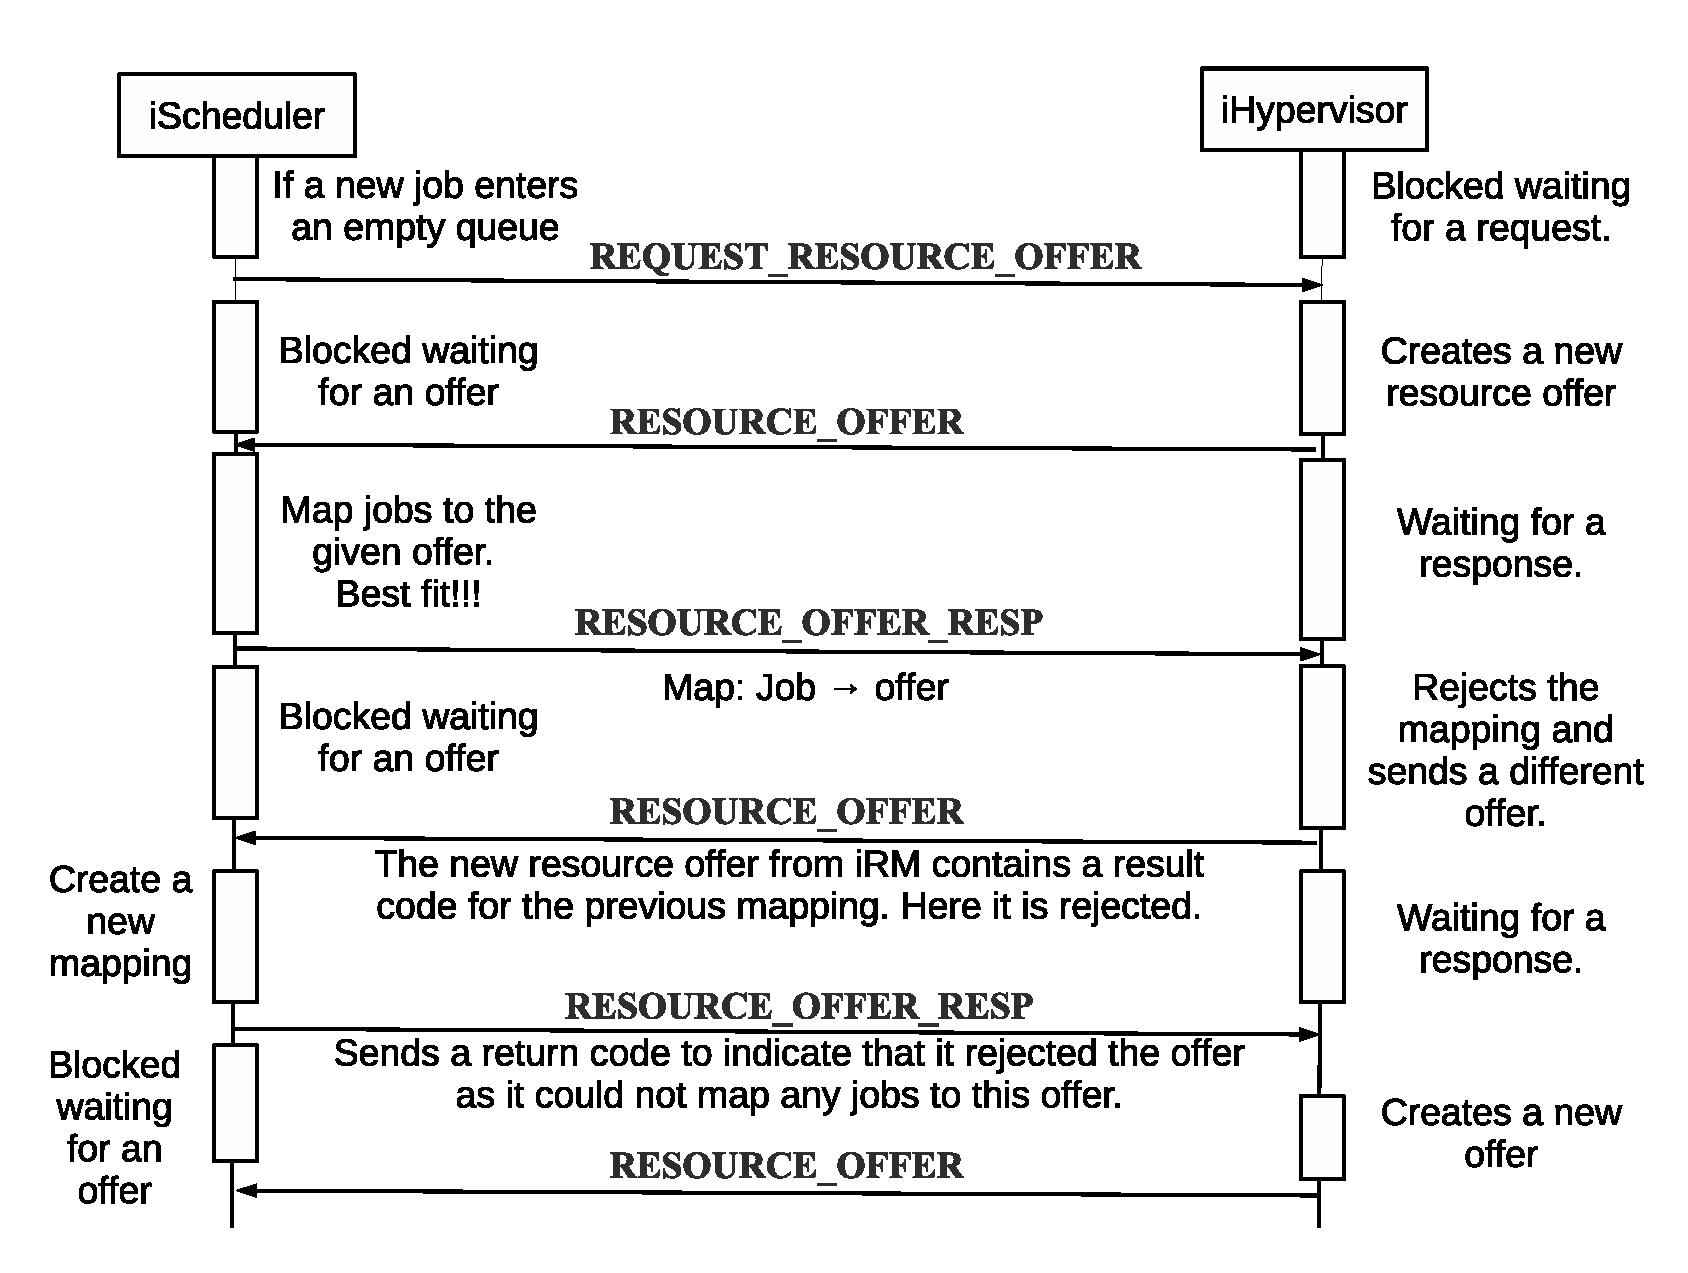
\includegraphics[width=1.0\textwidth, height=130mm]{./figures.eps}
\caption{Scenario 1}
\label{fig:Seq1}
\end{figure}
\clearpage
\begin{figure}[h]
\centering
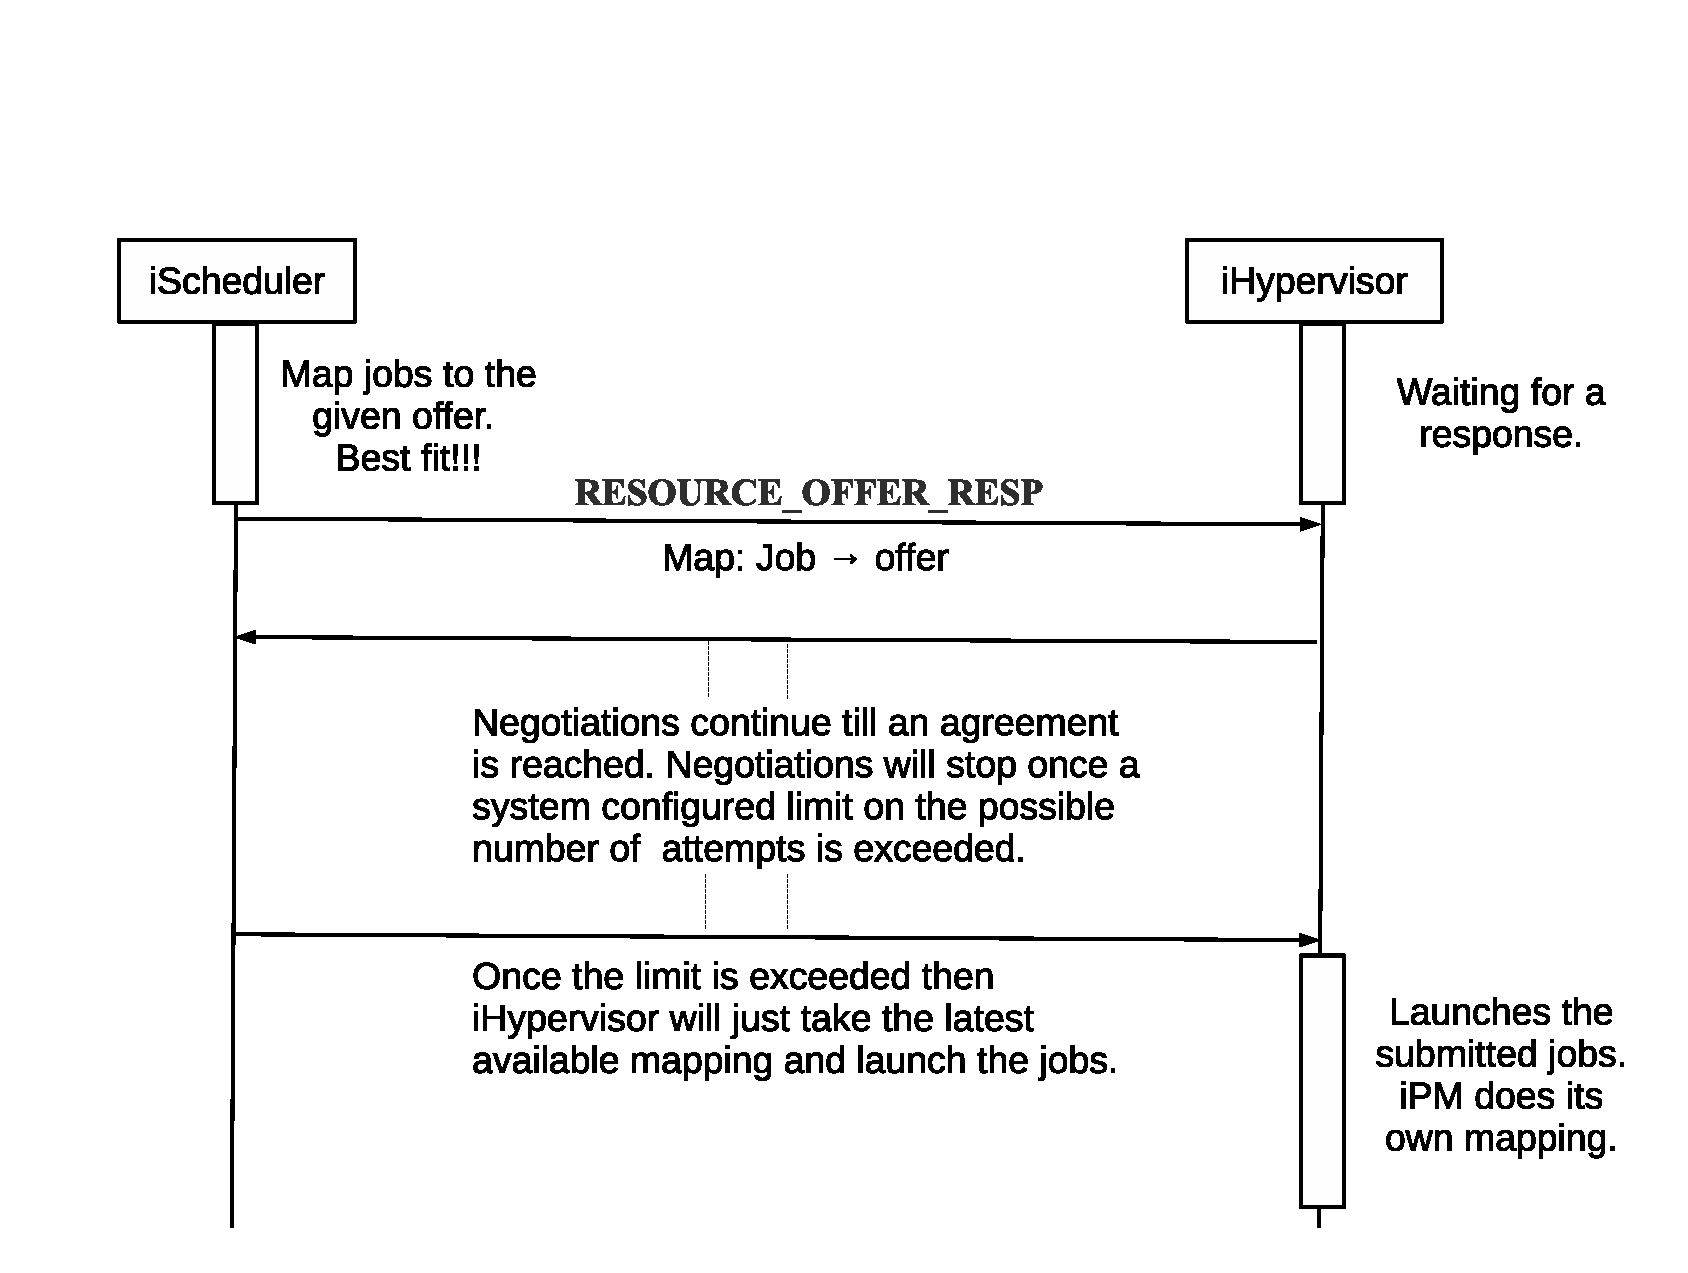
\includegraphics[width=1.0\textwidth, height=130mm]{./figures1.eps}
\caption{Scenario 1 contd.}
\label{fig:Seq1}
\end{figure}
\clearpage
\begin{figure}[h]
\centering
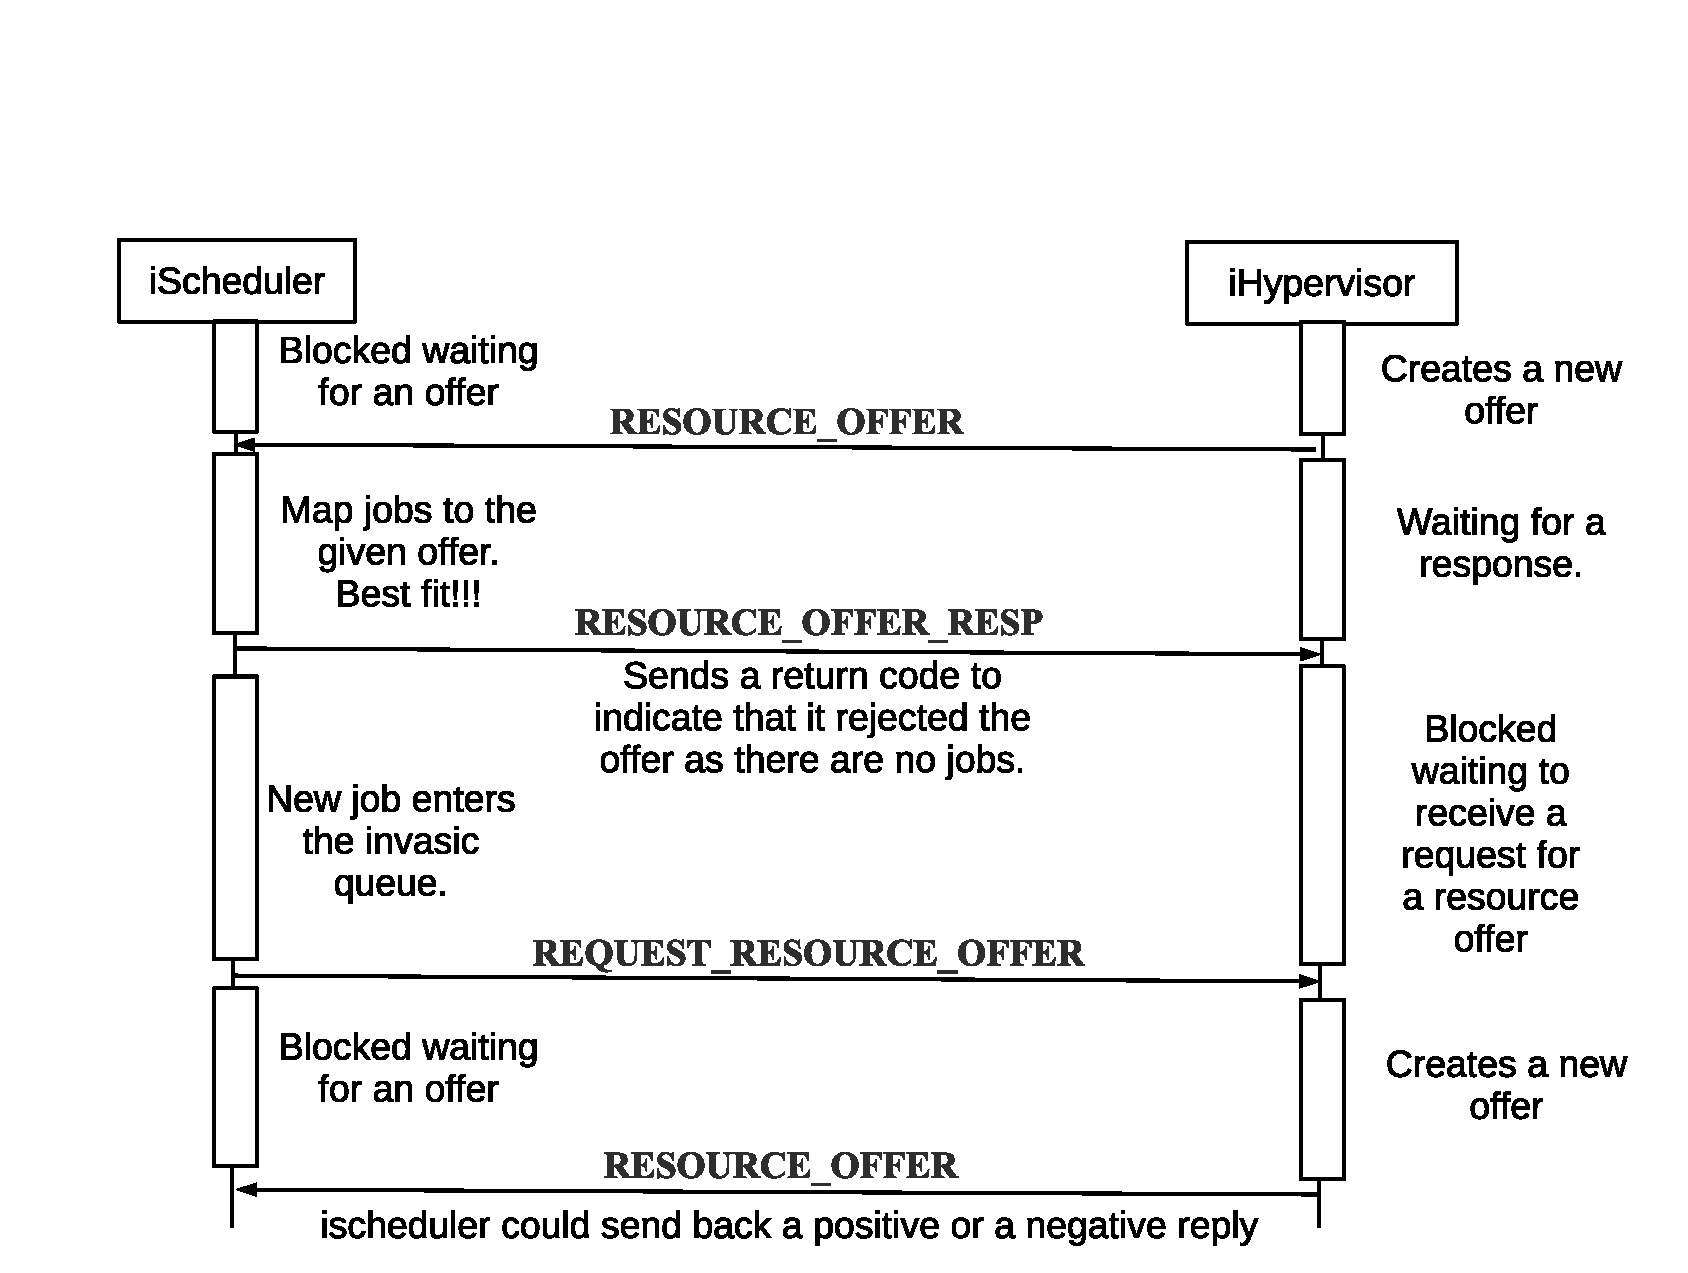
\includegraphics[width=1.0\textwidth, height=130mm]{./figures2.eps}
\caption{Scenario 2}
\label{fig:Seq2}
\end{figure}
\clearpage
\subsection{State Machine Diagrams}
\begin{figure}[h]
\centering
\includegraphics[width=1.0\textwidth, height=130mm]{./}
\caption{Protocol Initialization}
\label{fig:Seq2}
\end{figure}
\section{Conclusion}
\subsection{Scope for future work}
%\begin{figure}[h]
%\centering
%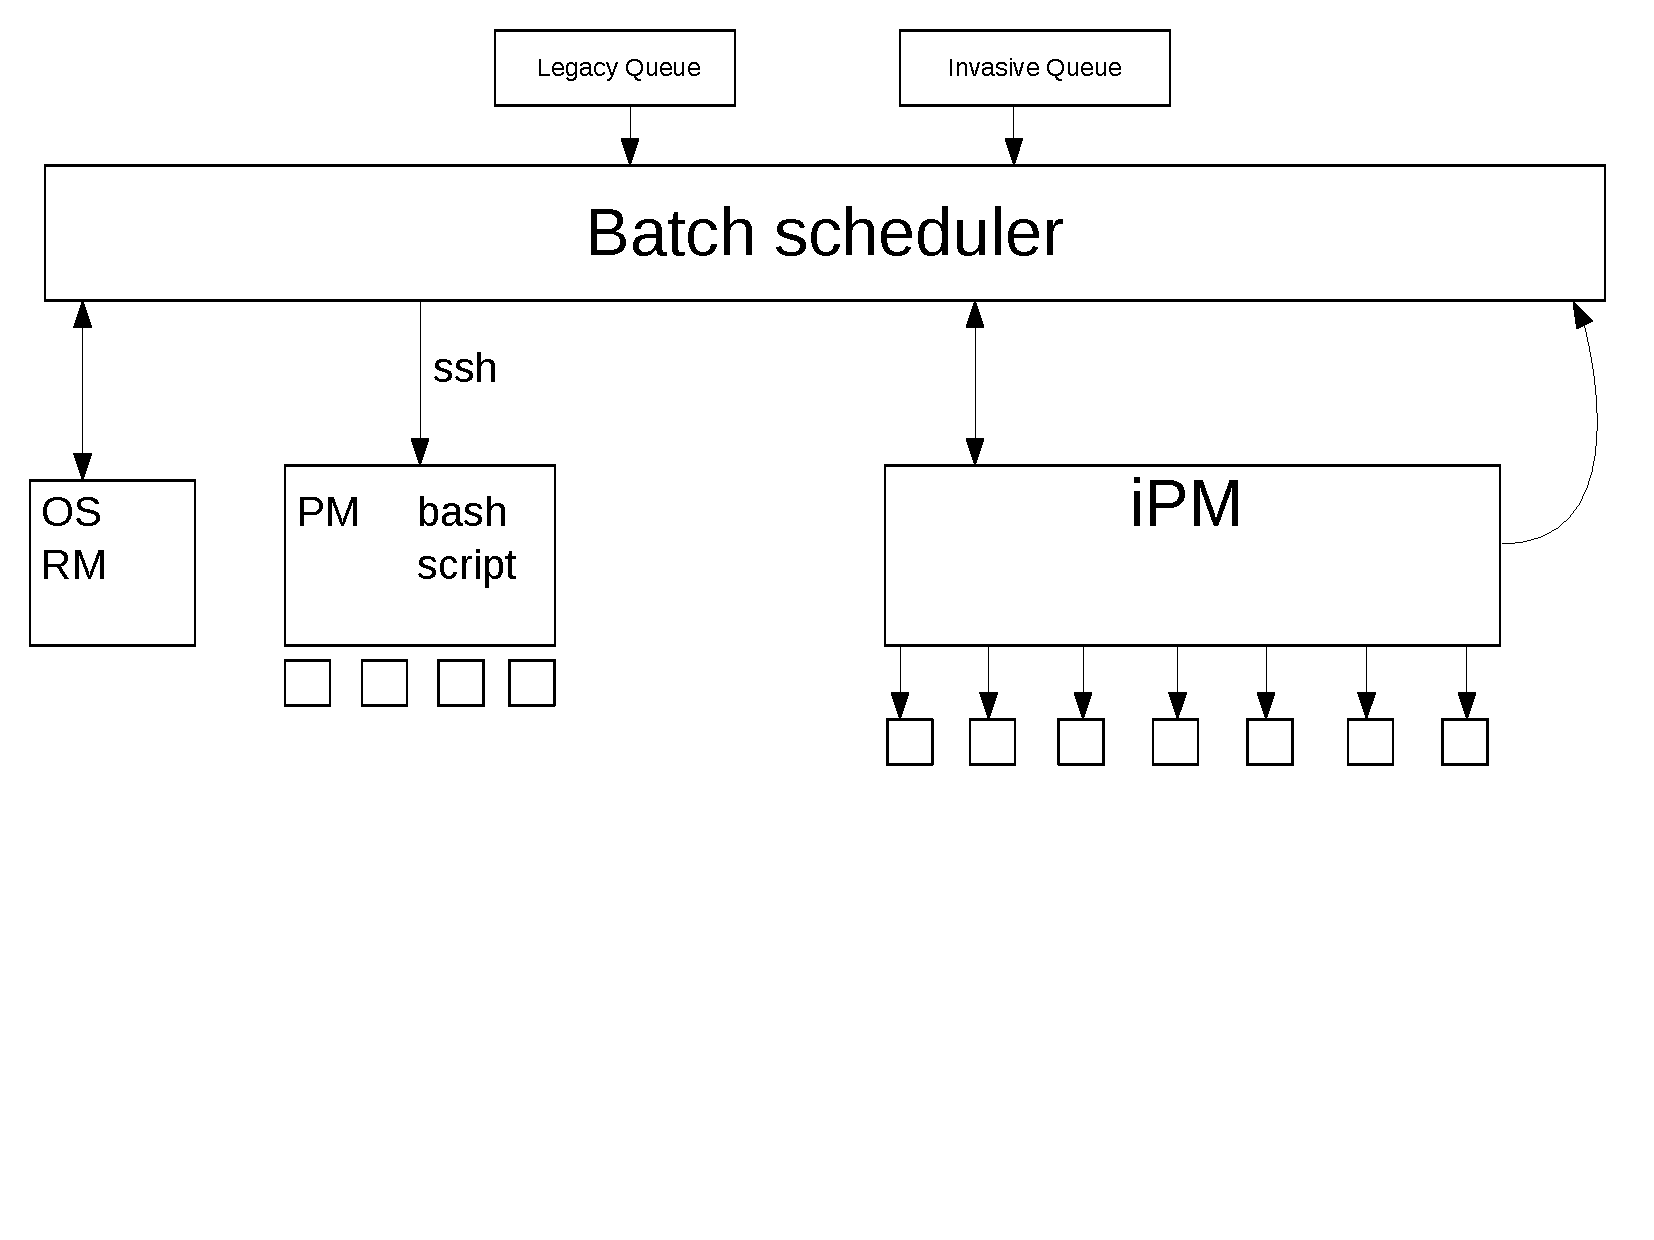
\includegraphics[width=0.65\textwidth, clip, trim=0mm 60mm 0mm 0mm]{data/architecture.pdf}
%\vspace{-0.15in}
%\caption{Invasive resource management architecture}
%\label{fig:arch}
%\end{figure}
\nocite{fontaine,gao,poorzahedy2,tianze,leblanc,kuo,poorzahedy1,wen}

\bibliographystyle{unsrt}
% Literature sources are to be found in seminarpaper.bib
\bibliography{nishanth}

\end{document}
